%  %% LyX 2.3.1 created this file.  For more info, see http://www.lyx.org/.
%  %% Do not edit unless you really know what you are doing.
%  \documentclass[twocolumn,english,showpacs,preprintnumbers,amsmath,amssymb,floatfix]{revtex4-1}
%  \usepackage[T1]{fontenc}
%  \usepackage[latin9]{inputenc}
%  \setcounter{secnumdepth}{3}
%  \usepackage{color}
%  \usepackage{babel}
%  \usepackage{graphicx}
%  \usepackage{esint}
%  \usepackage[unicode=true,
%   bookmarks=false,
%   breaklinks=false,pdfborder={0 0 1},backref=section,colorlinks=false]
%   {hyperref}
%  
%  \makeatletter
%  %%%%%%%%%%%%%%%%%%%%%%%%%%%%%% User specified LaTeX commands.
%  \hyphenpenalty=10000
%  
%  \makeatother
%  
%  \begin{document}
%  
\clearpage

\appendix 
\section{Defining $F_{2}^{charm}$ Beyond Lead Order}

\begin{figure}[t]
\centering
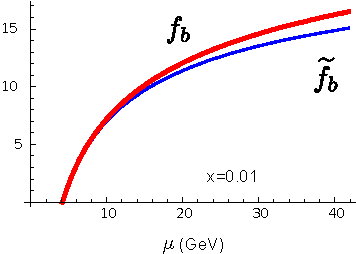
\includegraphics[width=0.45\textwidth]{./pics/fred/cancellation}
\caption{\textcolor{blue}{
We may switch to charm; I took from our heavy flavor paper.} 
The LO contributions correspond to the heavy quark ($Q$) initiated $f_{Q}$,
and the SUB to $\tilde{f}_{Q}$. The cancellation (LO-SUB) is quite
precise. If we were to remove LO or SUB, our TOT result would have
anomalous contributions (and correspondingly anomalous $\mu$-dependence)
in the region $\mu\sim m_Q$.}
\end{figure}


\begin{figure}[t]
\centering
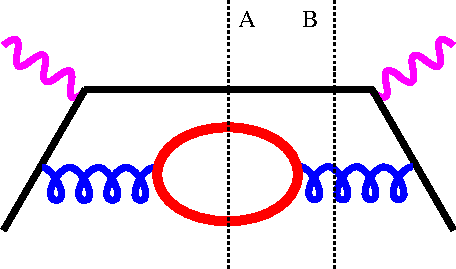
\includegraphics[width=0.45\textwidth]{./pics/fred/feyngraph}
\caption{\textcolor{blue}{draft in progress: } 
%
A higher order Feynman graph illustrating the difficulty in defining
an ``inclusive'' $F_2^{charm}$. 
If we have a light quark ($q$) scattering from a vector boson ($V$),
at higher orders we could have a charm--anti-charm loop. 
If we cut the amplitude with cut ``A'' we have charm in the final state
and this must be included in  $F_2^{charm}$. 
If we cut the amplitude with cut ``B'' there is no charm in the final state,
but this process is required to satisfy IR  divergences as governed by the Kinoshita-Lee-Nauenberg (KLN) theorem.
Also note, since this diagram contributes to the beta function, 
this highlights the difficulty of using an $\alpha_S$ and hard scattering $\hat{\sigma}$ with differing $N_{eff}$.
}
\end{figure}



\begin{figure*}
\centering
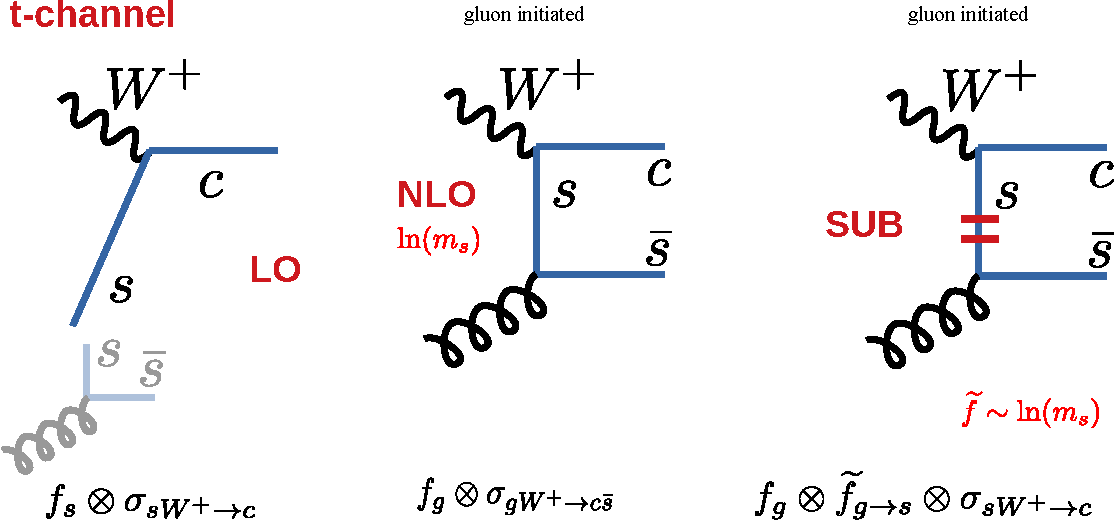
\includegraphics[clip,width=0.80\textwidth]{./pics/fred/tchannel}
\caption{Gluon NLO $t$-channel processes}
\end{figure*}
%
\begin{figure*}
\centering
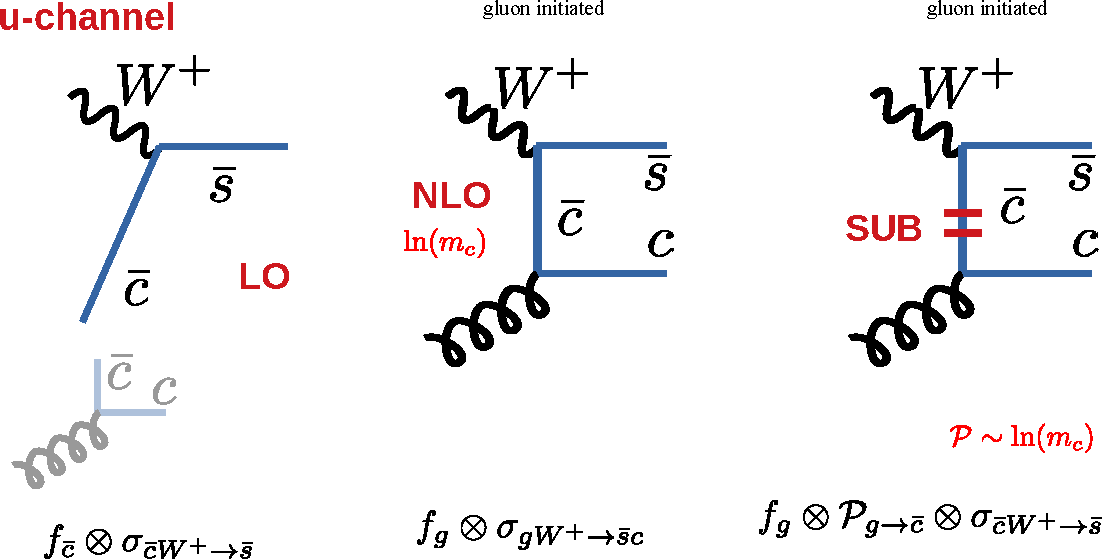
\includegraphics[clip,width=0.80\textwidth]{./pics/fred/uchannel}
\caption{Gluon NLO $u$-channel processes}
\end{figure*}


The charged current DIS charm production process involves some interesting
issues. Because two quark masses are involved $\{m_{s},m_{c}\}$,
we can separately examine the mass singularities of the $t$-channel
and $u$-channel separately; this separation is particularly useful
to understand how the FFNS and VFNS divide up the contributions to
the total structure function. Additionally, the DIS charm production
allows us to identify the deficiencies we encounter due to the fact
that a truly ``inclusive'' $F_{2}^{charm}$is not a theoretically
well-defined observable.

x

\textcolor{blue}{{[}FRED: THIS INTRO IS STILL ROUGH{]} Suppose we
attempt to compute the ``inclusive'' $F_{2}^{charm}$ for Charged
Current (CC) charm production at NLO in the VFNS. The obvious LO diagram
is $(sW^{+}\to c).$ What is not so obvious is we also will need ($\bar{c}W^{+}\to\bar{s}$).
This is because the $\bar{c}$ comes from a gluon splitting to $c\bar{c}$,
and the $c$ goes down the beam pipe along with the hadron remnants.
All three $u$-channel terms displayed in Fig.~{*}{*}{*} are required
for the result to be both i) insensitivity to the $\mu$-scale, and
ii) be free of mass singularities at large $Q^{2}$ scales; but this
requires measuring charm quarks in an experimentally unaccessible
region---the hadron remnants. This is why a truly ``inclusive''
$F_{2}^{charm}$ is ill-defined; it is experimentally unobservable.}\footnote{\textcolor{blue}{The proof of factorization for heavy quarks by Collins
cite{*}{*}{*}{*} addressed a fully inclusive $F_{2}$; it specifically
avoided the ill-defined $F_{2}^{charm}$. }}

\textcolor{blue}{What is actually measured experimentally is a differential
charm production process which must include a resolution scale (or
regulator) to make a cut on charm quarks in the beam fragments; this
``non-inclusive'' $F_{2}^{charm}$ (or ``exclusive'') measurement
can be well defined.}

\textcolor{blue}{For this discussion we will focus on the NLO gluon
initiated graphs; there are a parallel set of NLO quark initiated
processes, but the principles are fully illustrated by the gluon processes. }

\textcolor{blue}{Additionally, we note that an ``inclusive'' $F_{2}^{charm}$
in the FFNS is also ill-defined; at higher orders we have $g\to c\bar{c}$
processes which make it impossible to separate out a ``charm only''
contribution from the total $F_{2}$.}\footnote{\textcolor{blue}{See for example. Ref. Smith and van Neerven cite{*}{*}{*}
At ${\cal O}(\alpha_{S}^{3})$ we can have internal $g\to c\bar{c}$
processes which make a $F_{2}^{charm}$ definition ambiguous. This
issues is particularly problematic in beta-function which sums over
internal quark loops and determines the running of $\alpha_{S}$. }}

\subsection{t-channel at NLO}

The t-channel contributions at NLO are straightforward. We start with
a leading-order (LO) $sW^{+}\to c$ process. We then add the next-to-leading-order
(NLO) $gW^{+}\to c\bar{s}$ diagram; this exchanges an $s$ quark
in the t-channel, and thus will have a $\ln(m_{s}^{2}/Q^{2})$ divergence
for large $Q$. This is resolved by the subtraction (SUB) term $f_{g}\otimes{\cal P}_{g\to s}\otimes\sigma_{sW^{+}\to c}$
where the ${\cal P}_{g\to s}$ represents a perturbative splitting
of $g\to s$; the SUB term is proportional to ${\cal P}_{g\to s}\sim\frac{\alpha_{S}}{2\pi}\:P_{g\to s}^{(1)}\:\ln(m_{s}^{2}/Q^{2})$,
and will cancel the double counting between the LO and NLO graphs
in the limit where the exchanged $s$ quark becomes collinear.\footnote{Here we use ${\cal P}_{g\to s}$ to represent the perturbative splitting
contribution which at NLO is given by $\frac{\alpha_{S}}{2\pi}\:P_{g\to s}^{(1)}\:\ln(m_{s}^{2}/Q^{2})$,
where $P_{g\to s}^{(1)}$ is the usual DGLAP splitting kernel.} The logarithmic divergence (mass singularity) will cancel between
the NLO and SUB terms as $Q^{2}\to\infty$, resulting in a finite
result for the NLO t-channel contribution. 

\subsection{u-channel at NLO}

The u-channel at NLO is more subtle. We definitely need the NLO $gW^{+}\to c\bar{s}$
diagram with a $\bar{c}$ quark exchanged in the u-channel, and thus
will have a $\ln(m_{c}^{2}/Q^{2})$ divergence for large $Q$. This
is resolved by the subtraction term $f_{g}\otimes{\cal P}_{g\to\bar{c}}\otimes\sigma_{\bar{c}W^{+}\to\bar{s}}$
where the ${\cal P}_{g\to\bar{c}}$ represents a perturbative splitting
of $g\to\bar{c}$ and will cancel the double counting between the
LO and NLO graphs in the limit where the exchanged $\bar{c}$ quark
becomes collinear. Here, the SUB term is proportional to ${\cal P}_{g\to\bar{c}}\sim\frac{\alpha_{S}}{2\pi}\:P_{g\to\bar{c}}^{(1)}\:\ln(m_{c}^{2}/Q^{2})$.
The logarithmic divergence will cancel between the NLO and SUB terms
as $Q^{2}\to\infty$, resulting in a finite result for the NLO u-channel
contribution. 

\subsection{Why do we need the LO ($\bar{c}W^{+}\to\bar{s}$)?}

What is not so obvious is that we need the LO $u$-channel process
$\bar{c}W^{+}\to\bar{s}$.

Recall that it is essential we include the subtraction SUB term $f_{g}\otimes{\cal P}_{g\to\bar{c}}\otimes\sigma_{\bar{c}W^{+}\to\bar{s}}$
so that we get a finite answer at large energies $Q^{2}\to\infty$. 

At energy scales $Q\sim m_{c}$, the LO and SUB terms remove the double
counting between the LO and NLO processes. This is most apparent when
you plot the individual terms versus the $Q$ scale (or more properly,
it is the $\mu$ scale). {[}See Figure{]} In the region of $Q\sim m_{c}$,
the charm PDF $f_{c}$ (and hence, the LO contribution) rises very
quickly as it is driven by the very large gluon, and coupled with
a large $\alpha_{S}(m_{c})$. The SUB subtraction also rises quickly
as this is driven by the logarithmic term $\ln(m_{c}^{2}/Q^{2})$.
The difference LO-SUB is the physical contribution to the total (TOT=LO+NLO-SUB),
and it is this combination which is smooth across the ``turn on''
of the charm PDF. We now see that if we neglect the LO ($\bar{c}W^{+}\to\bar{s}$)
we loose the cancellation between LO and SUB in the $Q\sim m_{c}$
and our structure function (or cross section) would have an anomalous
shift at the location where we arbitrarily turn on the charm PDF. 

So to recap, the combination of the LO and SUB terms ensure a minimal
$\mu$-variation at low $\mu$ scales, and the combination of SUB
and NLO ensure the mass singularities are canceled at high $\mu$
scales. 

\subsection{FFNS: u-channel for $N_{F}=3$}

Let us clarify the case where we work in a FFNS with 3 flavors $\{u,d,s\}$
but no charm PDF. In this case there is no LO ($\bar{c}W^{+}\to\bar{s}$)
process as $f_{c}=0$, and there is no u-channel subtraction $f_{g}\otimes{\cal P}_{g\to\bar{c}}\otimes\sigma_{\bar{c}W^{+}\to\bar{s}}$.
This is all perfectly consistent. However, the NLO u-channel process
($gW^{+}\to c\bar{s}$) will have a potentially divergent $\ln(m_{c}^{2}/Q^{2})$
contribution from the exchanged charm quark; this is fine so long
as we don't go to large $Q$. If we do want large $Q$, then we will
need to resum the $\ln(m_{c}^{2}/Q^{2})$ logs using the charm PDF. 

We expect this FFNS to diverge from the VFNS result by contributions
proportional to $\sim\frac{\alpha_{S}}{2\pi}\:\ln(m_{c}^{2}/Q^{2})$.

\subsection{The bottom line: }

A truly ``inclusive'' $F_{2}^{charm}$ is ill-defined. Instead,
we necessarily must an ``experimentally'' defined $F_{2}^{charm}$
where we specify conditions so that the final state charm is isolated
from the hadron remnants. 

We can talk about a fully inclusive $F_{2}$ where we include all
flavors; this was the subject of Collins' proof. 

If we compute a ``pseudo-inclusive'' $F_{2}^{charm}$ in the Variable
Flavor Number Scheme, we do need to include the LO ($\bar{c}W^{+}\to\bar{s}$)
and the associated SUB ($gW^{+}\to c\bar{s}$).

We can compute in the Fixed Flavor Number Scheme, but in the large
energy limit, we encounter $\ln(m_{c}^{2}/Q^{2})$ divergences. In
practice, our $Q$ scales are not large enough to generate infinities,
but they are large enough where we see the resummed logs included
in the VFNS charm PDF become important. Regardless, the FFNS is also
unable to define a truly ``inclusive'' $F_{2}^{charm}$.

%\end{document}
